This chapters explains the related work that is helpful in understanding the concepts, mathematical constructs, terms, and definitions that are necessary to understand the working details of the thesis. The first part discusses Physical(ly) Unclonable Functions, second part introduces the concept of the BCH code, third part talks about Golay code constructs and finally a synopsis of Jaccard Index is presented.

\section{Physical(ly) Unclonable Functions - Background}
In order for the reader to have a better understanding of the fundamentals of Physical(ly) Unclonable Functions, this section discusses some basics of PUFs. Initially the historical emergence of PUFs is presented, followed by a general definition of the PUF. Then the PUFs are classified and a selection of different types of PUFs is presented. Lastly, the basics of linear codes like BCH and Golay codes are discussed that form the basis for the fuzzy extractor. Work in this section is mostly derived
from \cite{17,18}.\\

\subsection{History and origins}
Physical(ly) Unclonable Functions (PUFs) are based on unique and non-reproducible artifacts, which were caused by production variances during manufacturing processes. PUFs were first presented in the early eighties \cite{16}. Fingerprint identification of humans goes back to at least nineteenth century \cite{th21} and from that emerged the field of biometrics. In the twentieth century, random patterns in paper and optical tokens were used for exclusive identification of currency notes and strategic arms \cite{2,8,53}. A
formalization of this concept was introduced in the beginning of the twenty-first century. In 2001, Pappu et al. \cite{19,39} presented \emph{physical one-way functions}. The next year 2002, Gassend et al. \cite{21} proposed a silicon-based PUF approach as a \emph{physical random function}. This led to coining of the acronym PUF (\emph{Physical(ly) Unclonable Function}) to avoid confusion with the concept of pseudo-random functions (PRF), which was an already established concept in cryptography.\\

The promising properties of PUFs like physical unclonability and tamper evidence which are favorable for security mechanisms, led to the increase in popularity of PUFs and in coming years new types of PUFs were proposed. Due to their practical usages and encouraging properties the interest in PUFs has risen significantly; they are still a hot topic in the field of hardware security and can contribute to the evolution of security mechanism and applications.\\

\subsection{Definition}
The definition of PUFs is taken from Gassend et al.\cite{21}:

\emph{A Physical(ly) Unclonable Function (PUF) is a function that maps challenges to responses, that is embodied by a physical device, and that verifies the following properties:\\
1. Easy to evaluate: The physical device is easily capable of evaluating the function in a short amount of time.\\
2. Hard to characterize: From a polynomial number of plausible physical measurements (in particular, determination of chosen challenge-response pairs), an attacker who no longer has the device, and who can only use a polynomial amount of resources (time, matter, etc.) can only extract a negligible amount of information about the response to a randomly chosen challenge.\\}

To simplify, PUFs are functions that use hardware manufacturing process variations to generate a random output. They are easy to evaluate which means that for a given input, the result is extracted without much effort. Unclonable keyword implies the output function cannot be duplicated to make another PUF. Random response means it contains an equal number of ones and zeros.

\subsection{PUF terminologies}
This section introduces commonly used terms used for describing PUFs and their characteristics. Work in this subsection is inspired from \cite{thbook}

\subsubsection{Challenge and Responses}
As discussed in the definition, PUF produces output on being queried with an input. Since the input may have more than one possible output so PUFs are not functions in a mathematical sense rather they are considered function in engineering sense i.e a procedure performed by or acting upon a specific (physical) system. \cite{thbook}. The input to PUF is called \emph{Challenge} and output is termed as \emph{Response}, together they are known as \emph{Challenge-Response Pair} or \emph{CRP} and
the relation imposed between challenges and responses by a particular PUF is called as its \emph{CRP behavior}. PUF is applied in two phases, the first phase is \emph{enrollment}, where a certain number of CRPs are collected from a PUF and stored in a \emph{CRP database}. In the second phase called \emph{verification}, a challenge from CRP database is applied to the PUF and the produced response is compared with the corresponding response from the database (section 2.1 \cite{thbook}).

\subsubsection{Intra- and Inter-Distance metrics}
\label{intra_inter_section}
The concept of inter-versus intra-(class) distance is inherited from the theory of classification and identification:
\begin{itemize}
	\item for a specific challenge, inter-distance between two PUFs instances is the distance between two responses produced by applying the same challenge to both PUFs.
	\item for a specific challenge, the intra-distance between two evaluations of the single PUF is the distance between two responses produced by applying the same challenge twice to the same PUF. (section 2.2 \cite{thbook})
\end{itemize}

In our case, we deal with challenges and responses that are output in bit strings (after decoding and quantization of analog physical stimuli and measured effect), so Hamming Distance is a good metric to measure the difference in the responses i.e. degree by which the responses from the same challenge differ. To amplify the Hamming distance it is often expressed as a fraction of the length of the considered strings, in that case it is known as \emph{fractional Hamming distance}

\subsection{Reliability Issues}
As pointed out earlier in the introduction, PUF is sensitive to external factors and therefore the output of PUF is not consistent. These factors can be inevitable random noise or measurement uncertainties which give rise to the intra-distance between PUF responses (section 2.3 \cite{thbook}). Apart from these undesirable effects PUFs are susceptible to other sources of noise e.g. varying temperature or supply voltage on PUFs integrated circuit, these factors contribute to a \emph{systematic} effect on
response measurement. Another cause for unreliable responses is the \emph{aging effect}, which causes gradual degradation of the device resulting in varying PUF responses. Consequently, PUF responses need post-processing techniques to be applicable in practical security scenarios. One such case is extracting a reliable key from PUF that requires a scheme called Fuzzy Extractor (covered in more detailed in later section \ref{fuzzy_section}).

\subsection{Classifications}
The popularity of PUFs and immense research on the topic has resulted in various concepts and constructions, we talk about the ones that are concerned with this thesis and for completeness briefly describe other classifications.\\
The following sections talk about the classification of PUFs that are subdivided into three different groups based on \cite{17}:
\begin{enumerate}
	\item Implementation technology and material of the proposed construction
	\item A more general set of physical construction properties
	\item Algorithmic properties of the challenge-response behavior
\end{enumerate}

The first criterion for classification is the implementation technology of the construction. PUFs can be realized with different technologies and materials like glass, plastic, paper, electronic components and integrated circuits (ICs). Essentially there are two classes in this group based on the \emph{electronic} nature of the identifying features.\\

\textbf{Non-electronic PUFs} are PUFs where the nature of the components in the system that contributes to the random physical microstructure of unique PUF is of non-electronic origin. It should be noted that keyword 'non-electronic' only reflects the origin of the PUF behavior, post-processing (like fuzzy extraction) or intermediate steps can be electronic. Examples can be Optical PUFs where the core element is an optical microstructure constructed by mixing
microscopic refractive glass spheres in a transparent epoxy plate (section 3.1.1 of \cite{thbook}). A unique response is obtained upon irradiating the transparent material with a laser, this can be interpreted as a PUF response. Another example are Paper-based PUFs where the random fiber structure of the paper is scanned using a laser. The reflection from the erratic fiber serves as a unique identifier and can be considered as a PUF response \cite{thbook}.

\textbf{Electronic PUFs} proposed construction contains random variations derived from electronic properties of the underlying material e.g. resistance, capacitance etc. \emph{Silicon PUFs} are a major subclass of electronic PUFs. They were the first practical realization of PUFs introduced by Gassend et al. \cite{21}. Since Silicon PUFs can be connected to the integrated circuit on the same chip, they can be instantly deployed as hardware building block in cryptographic implementations. \cite{17}.
Another example is a construction called RF-DNA where copper wires are arranged randomly on a silicone medium to generate PUF responses.\\

The second classification which is based on the construction properties subdivides the PUFs in \textbf{Intrinisic PUFs} and \textbf{Non-Intrinsic PUFs}. Initially proposed by Guajardo et al. \cite{11}, \emph{Intrinsic PUFs} must meet following two conditions:
\begin{itemize}
	\item the evaluation of the PUF is performed internally (the measurement instrument is integrated into the device).
	\item the random instance specific features are implicitly imported during its manufacturing process.
\end{itemize}

We look with some detail in the above two conditions. First one states that the evaluation, which is a physical measurement, can be internal or external. An external evaluation is the measurement of features that are externally observable and is done with the help of equipment external to the physical entity. Internal evaluations, on the other hand, are measurements of features that are internal to the instance and is performed by equipment absolutely embedded in the instance itself. There are some
advantages for internal evaluations, one there is a less security risk since the measurement entity is embedded in the instance and the PUF response is protected from the outside world. Also, there is a practical leverage because every PUF instance can evaluate itself without any external restriction. Hindrance from outside influences and measurement errors are also minimized in the internal evaluation. With \emph{Non-intrinsic PUFs}, the external measurement can pose a security
hazard if an adversary observes the PUF response.\\

The second one distinguishes between the source of the random variations. The manufacturer can explicitly add randomization procedure to introduce random features that are later measured during PUF evaluation or measured random features can be an implicit side-effect introduced during the production of the integrated circuit and PUF instance. This means they arise naturally and cannot be controlled by the manufacturer, hence even he/she cannot reproduce and clone the same random features. These
implicit random variations incorporated during manufacturing are called \emph{process variations} come at no extra cost, so they incur no additional cost and are attractive from economic viewpoint.\\

The final classification is based on the Challenge-Response behavior security properties. Guajardo et al. \cite{11} introduced the concept of \textbf{Strong} and \textbf{Weak PUFs} which was further expanded by Rührmair et al.\cite{29}. They state that a Strong PUF is a PUF that an adversary can have access to for a long period of time and still he/she cannot uncover the working of the PUF function or how the PUF is evaluated to map to a specific response. In other words, we can still come up with a
new challenge that the adversary does not know what the response to it will be. Consequently, this implies that:
\begin{itemize}
	\item the considered PUF has a very large challenge set, or else the adversary can apply brute force to know responses to all challenges.
	\item it is not possible to know the mapping function between CRPs based on observed CRPs, that means PUF is unpredictable.
\end{itemize}
PUFs that are not \emph{Strong PUFs} and those which have a small challenge set are called \emph{Weak PUFs}. Naturally Strong PUFs are favored in a good securely designed application as compared to Weak PUFs. However, construction of such a Strong and practical (intrinsic) PUFs is rather difficult and still an open problem \cite{29}.\\

\subsection{PUF types}
This section presents a selection of different PUF constructions according to \cite{17}. The general working principles of different PUF realizations are explained accompanied with security-related information.

\subsubsection{Arbiter PUFs}
\label{arbiterpuf}

Lee et al.\cite{31} proposed arbiter PUF as a delay-based silicon PUF. The idea is to have two digital paths with random process variations and explicitly introduce a race condition between signals that flow via these digital paths. The paths end in an arbiter circuit that referees the race i.e it resolves which of the paths was faster and correspondingly outputs a binary bit. It is made sure that both paths are designed to have (nearly) same nominal delays, therefore the result of the race and hence
response of the arbiter cannot be precisely determined based on the design. As we discussed even after having almost identical nominal delays, the delay experienced by the signal is a random delay that a side effect (in our case the desired effect) of the random silicon process variations on the delay parameters. This silicon process variation is random per device but static for a particular PUF device. So we can have the arbiter circuit device specific random response as the basis for the PUF
behavior.\\

In case both paths happen to have same nominal delays (due to complex nature of the electronic circuitry and used gates), both signals arrive almost synchronously at the arbiter in which case arbiter circuit goes in a \emph{metastable state} and logic output of the arbiter circuit is temporarily unknown (electronically, voltage of arbiter output is between levels for a logic high and low). After a short random backoff time arbiter switches from its metastable state and outputs a random binary
value not dependent on the conclusion of the race, but in this case, the output of the arbiter is not device-specific and not static. This phenomenon is the origin of unreliability (noise) of the responses in an arbiter PUF.\\

The implementation of arbiter PUF consists of two delay paths which contain a chain of switch blocks that connects two input signals to its two outputs either in a cross or straight configuration. This configuration is modifiable via a configurable selection bit. The Figure \ref{img:arbiter} shows the inner cross-section of the switches, which are logically implemented as 2-to-1 multiplexers (muxes). A total n number of switch blocks are linked with each block having a selection bit (n configuration bit-vector) to
configure a total of 2$^n$ possible delay path pairs. This n-bit vector is considered as a challenge, and the random process variations in the delay paths make sure that the input-output delays are different and each of the 2$^n$ paths leads to a race to be resolved by the arbiter circuit. The final output bit from the arbiter is considered as a response to the PUF challenge. Arbiter circuit can be implemented as a simple SR NAND latch or some other digital latch/flip-flop. Following two conditions are
important to determine if the PUF response depends individually on process variations or on the delay parameters:
\begin{itemize}
	\item the delay paths are designed to be symmetrical, the cause of any difference is process variation.
	\item arbiter circuit must not be biased for one input over other.
\end{itemize}

\begin{figure}
	\centering
	\fbox{ 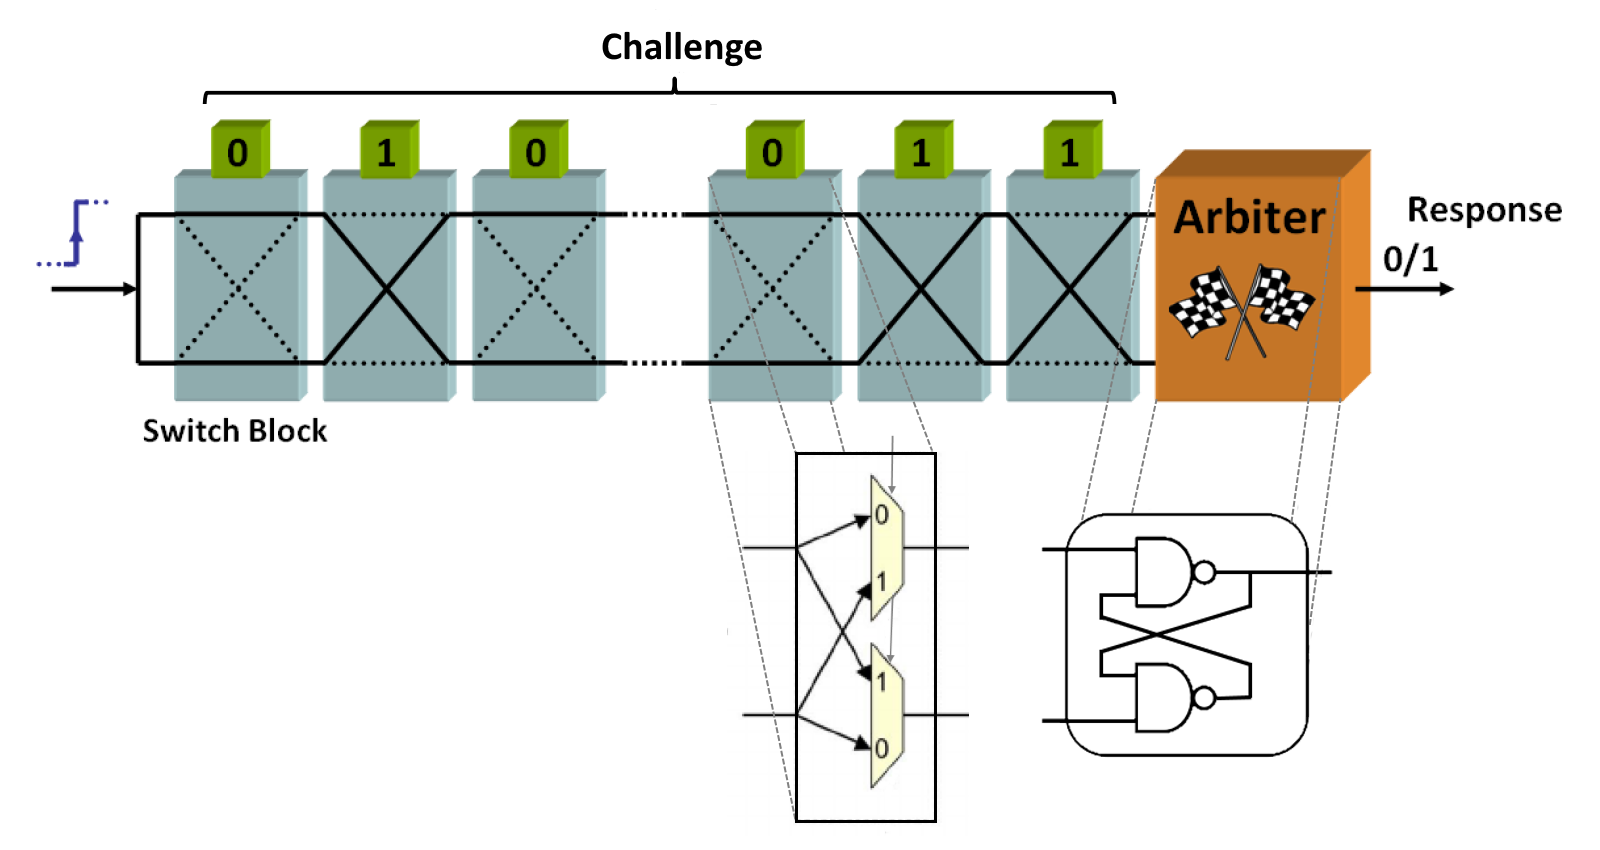
\includegraphics[width=0.9\textwidth]{images/arbiter_4.png}}
	\caption{Construction of a basic arbiter PUF, \emph{switching blocks} realized with muxes and an \emph{SR latch} realized with NAND gates, modified graphic based on \cite{17,18,38}}
	\label{img:arbiter}
\end{figure}

\textbf{\emph{Security Issues:}}
Though the challenge set is large still the number of delay parameters which effect the PUF response are linear in n, hence the 2$^n$ challenges cannot generate independent responses. A certain model or mathematical clone can be built for a given arbiter PUF if the adversary learns the underlying delay parameters. This clone can accurately forecast the PUF responses rendering the arbiter PUF hackable in security applications scenarios. Machine learning techniques like artificial neural
networks (ANNs) and support-vector machines (SVMs) can be employed to implicitly learn the underlying delay parameters by observing the challenge-response pairs.

\subsubsection{SRAM PUFs}
\label{srampufs}
The concept of an SRAM PUF was introduced by Guajardo et al. \cite{11} and Holcomb et al. \cite{50} in 2007. Static Random-Access Memory (SRAM) is a digital memory technology based on bistable circuits. (section 2.4.4 of \cite{17}). It consists of six MOSFETs transistors, out of which four are contained in two inverters. Each inverter comprises of one p-MOS and one n-MOS MOSFET. As you can see from Figure \ref{img:sram} the inverters are cross-coupled at the SRAM cell's core. In the terms of mathematical logic, the circuit has two stable states (bistable), each state represented by a binary
digit (0 or 1) that is stored in the cell. Two MOSFETs are used to read and write the cell contents. An SRAM cell is volatile and does not store its state on power-off.\\

\begin{figure}
\centering
\fbox{ 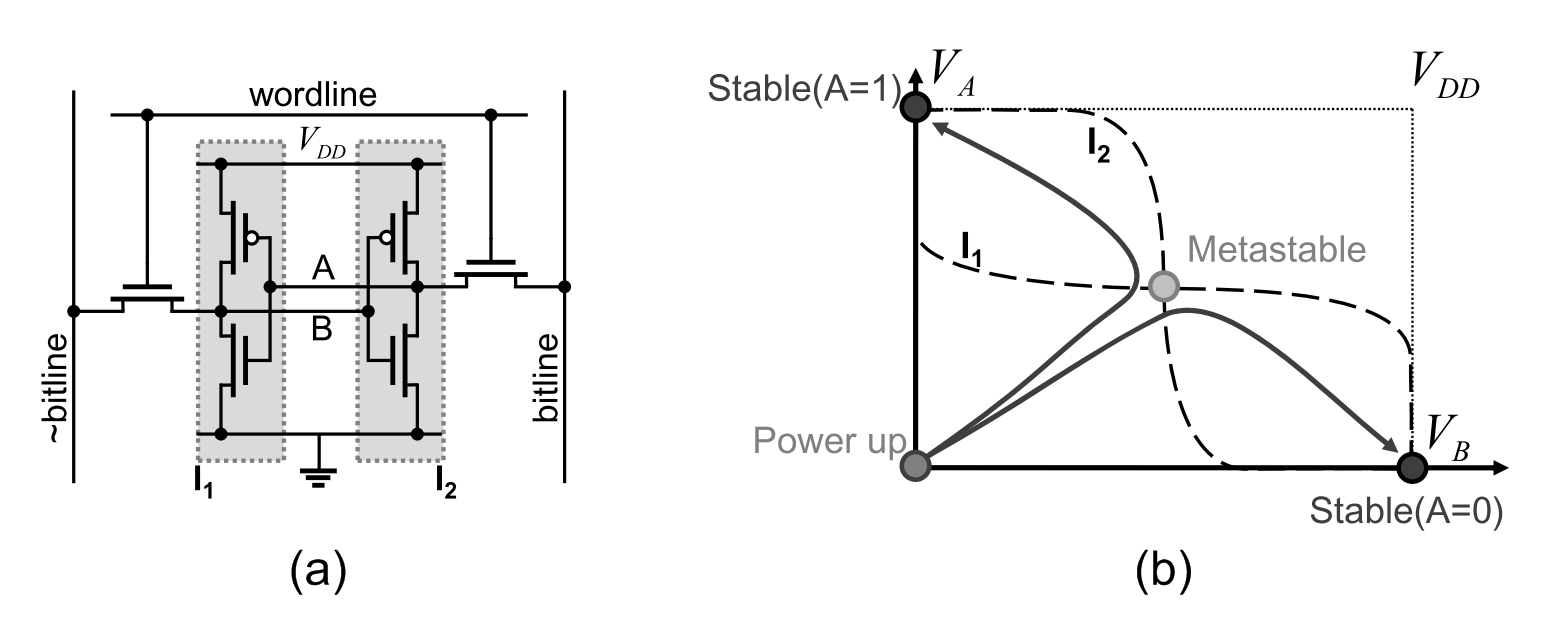
\includegraphics[width=0.9\textwidth]{images/sramPUF.png}}
\caption{(a) Construction of a standard CMOS SRAM cell circuit, (b) initial voltage transfer curves  \cite{17}.}
\label{img:sram}
\end{figure}

There are three possible operating points, two are stable and one is metastable as shown in Figure \ref{img:sram}. The deviation from stable points is automatically restored to its original point due to the feedback from the circuit. Adversely any deviation from a metastable point is amplified by the positive feedback from the circuit and cell moves to either of the stable points. After the supply voltage $V_{DD}$ comes up, the cell shifts to one of the preferred stable points, which is determined by the difference in
strength (device mismatch) of the MOSFETs in the cross-coupled inverter circuit. Due to performance and efficiency reasons, the inverters are designed to be perfectly in sync, the device mismatch is a result of the random process variations in the silicon production process. This random preferred initial operating point is unique to a specific cell. For a small mismatch, the preferred initial stable point is determined by the sign of the mismatch, though voltage noise can render the cell to
power-up in a non-preferred state. Finally the cells with almost zero mismatch power-up in the metastable state and shift to one of the stable points randomly.\\

Most SRAM cells have strongly preferred cell-specific initial state due to the magnitude of the process variations on the device mismatch; only a small number of the cells have weakly preferred or no preferred state, hence a typical SRAM cell exhibits strong PUF behavior. These cells are arranged in a large array giving millions of response bits, challenge for this cell assembly is the address of the cell.\\

\subsubsection{Ring Oscillator PUF}

\begin{figure}[t!]
\centering
\fbox{ 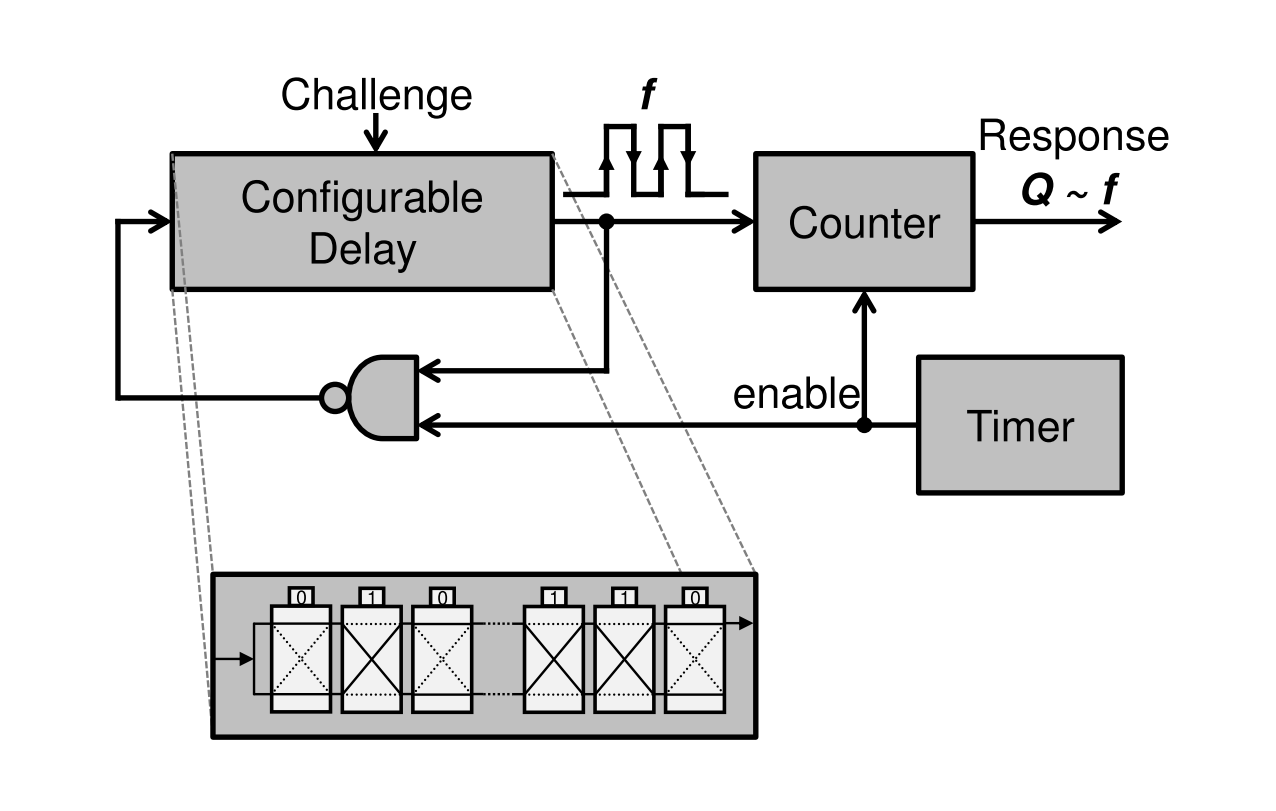
\includegraphics[width=0.9\textwidth]{images/ringPUF_1.png}}
\caption{Construction of a basic ring oscillator PUF as proposed by Gassend et al. \cite{21,17}.}
\label{img:ring}
\end{figure}

\begin{figure}[h!]
\centering
\fbox{ 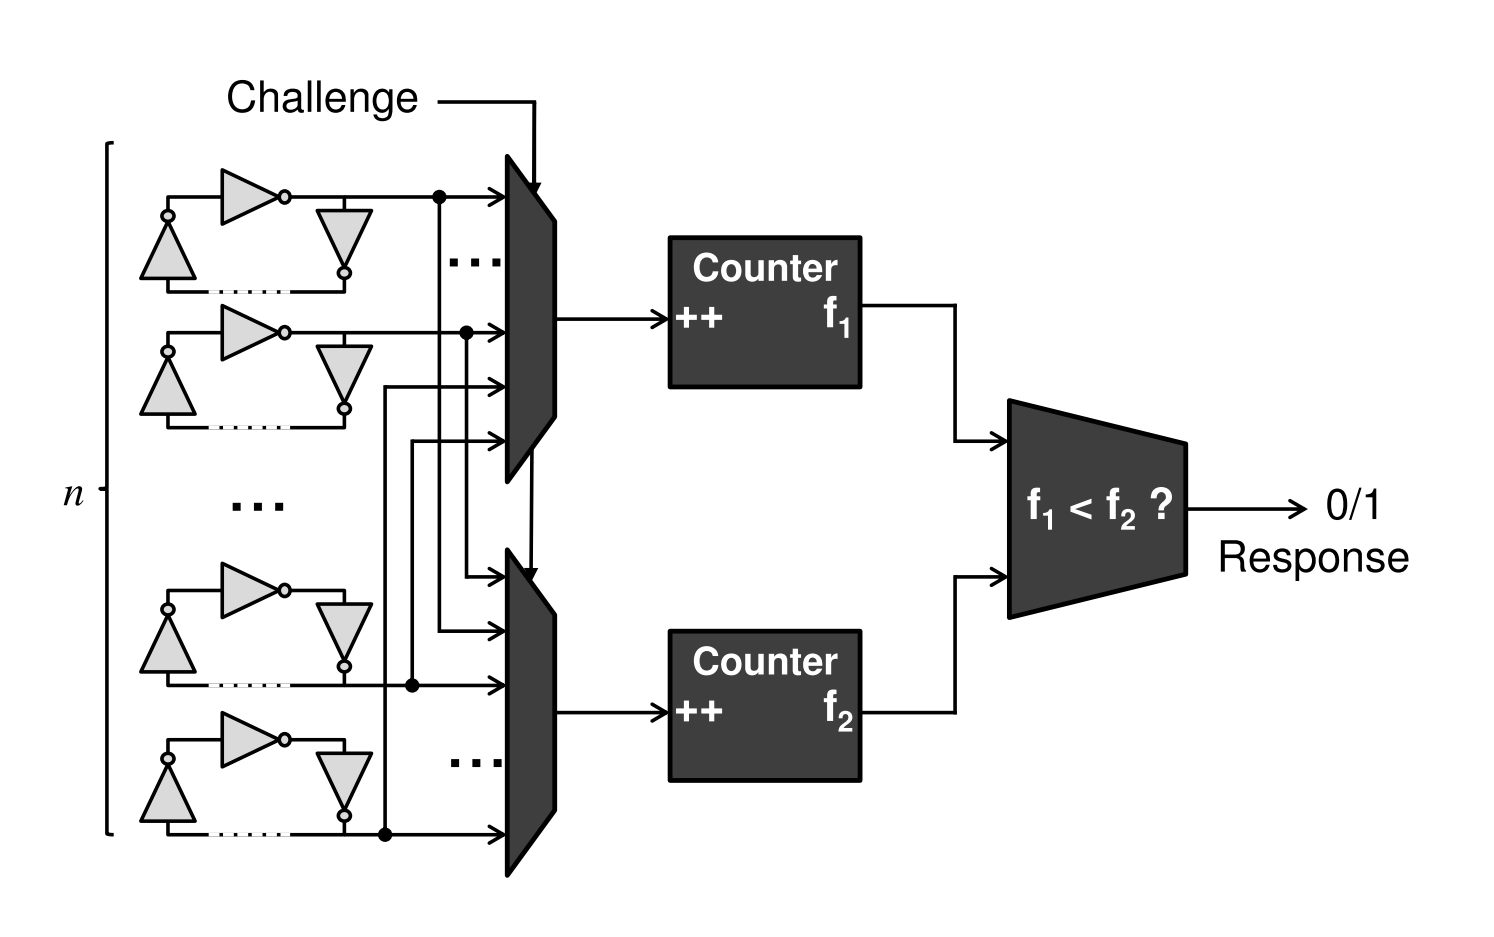
\includegraphics[width=0.9\textwidth]{images/ringPUF_2.png}}
\caption{Construction of a ring oscillator PUF as proposed by Suh and Devadas \cite{8,17}.}
\label{img:ring_suh}
\end{figure}

Proposed by Gassend et al. \cite{21} it is another type of delay-based intrinsic PUF. There are two parts to ring oscillator PUF, first is the ring oscillator and other is the frequency counter which are arranged in a configuration as shown in the Figure \ref{img:ring} and connected to a response generating algorithm. Gassend et al. uses a variant of the switch block base delay line similar to arbiter PUF \ref{arbiterpuf} which is transformed in an oscillator with the help of a negative feedback.
An AND gate is added to turn off/on the oscillation, which is fed to a frequency counter that counts the number of oscillating cycles in a fixed time interval. The same setup for ring oscillator on another device with the same implementation has different counter value because of the silicon process variations which forms the basis of the PUF response.\\

There are some other side effects associated with ring oscillator PUFs, one of them is significant influence from the environmental conditions like temperature changes and voltage fluctuations. The frequency changes introduced by these factors outweigh the deviations caused by the process variations, so to counteract these changes we need a post-processing technique known as \emph{compensated measuring}. The main idea is to calculate the ratio of the frequency of two ring oscillators
on the same device since they both are affected by identical environmental factors, hence the ratio would be more uniform. According to observations average intra-distance between evaluations is approximately 10\% and the average inter-distance is approximately 50\% (section 2.4.2 \cite{17})

\subsubsection{Optical PUFs}

Even before the introduction of PUFs an unclonable identification system based on random optical reflection patterns was proposed in \cite{th53}. Proposed by Pappu et al. as Physical One-Way Functions (POWFs), optical PUFs contain a microstructure constructed by blending microscopic (500 $\mu$m) refractive glass spheres in a miniature (10 x 10 x 2.54 $mm$) transparent epoxy plate. This token is illuminated with a helium-neon laser which produces an irregular wavefront;
the cause for this irregularity is the multiple scattering of the laser by the refractive particles. Finally, a CCD camera captures the speckle pattern and digitally processes it by applying Gabor hash to it as a feature extraction procedure (section 3.1.1 of \cite{thbook}). The final output is a string of bits that deviates significantly if the orientation of the laser beam is even minutely changed.\\

The PUF challenge is made up from the exact positioning of the laser and the resulting Gabor hash of the emerged speckle pattern is considered as a response. The operation and implementation for optical PUFs are shown in Figure \ref{img:optical}. A number of experiments were performed in \cite{19,39} for testing the characteristics of the optical PUFs and the following text summarizes their results. The values are taken from \cite{19,39}. In total, four optical tokens were used with 576
individual challenges, to calculate the PUF responses. Intra- and inter-Hamming distances were evaluated with an average inter-distance of $\mu_{inter}$ = 49.79\% and average intra-distance of
$\mu_{intra}$ = 25.25\%. One of the main limitations of such an optical PUF is the burdensome large setup consisting of a laser and mechanical positioning system. They are classified as non-electronic, non-intrinsic and strong PUFs.\\

\begin{figure}
\centering
\fbox{ 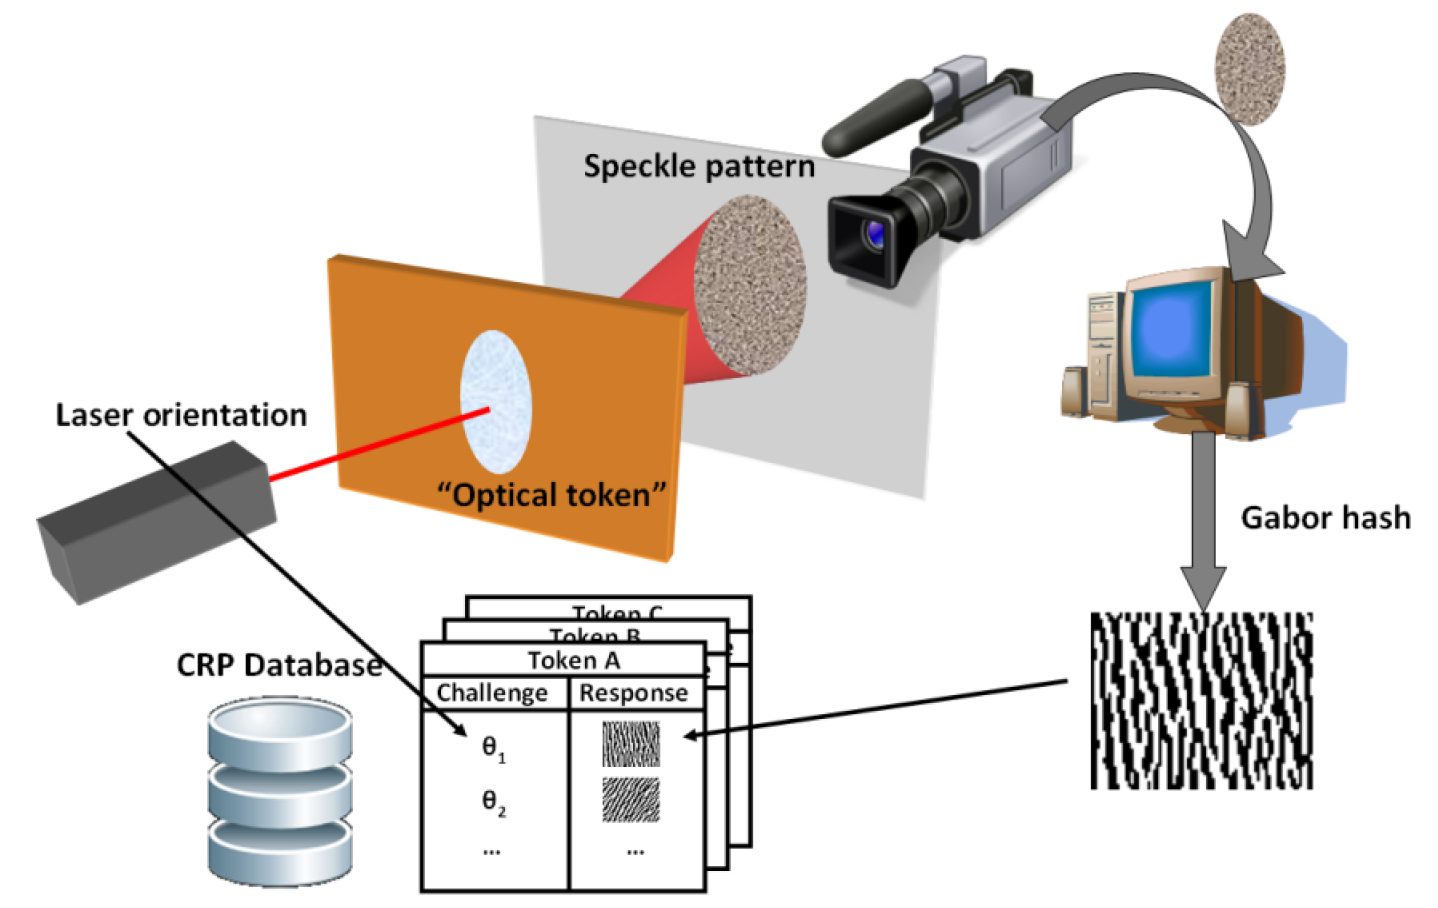
\includegraphics[width=0.9\textwidth]{images/opticalPUF.png}}
\caption{Construction of a basic optical PUF as proposed by Pappu et al. \cite{18,19}.}
\label{img:optical}
\end{figure}

\section{Linear Codes, BCH and Golay Codes}
In order to understand the working of the toolkit and fuzzy extractors (discussed later in section \ref{fuzzy_section}), we need to look at two specific types of linear codes. The following sections discuss the basics of linear codes and their mathematical constructs. After the initial explanation of what linear codes are, we go on to explain BCH codes and Golay codes that are used in the PUF toolkit to extract private and public keys in conjunction with PUFs. The second part
gives the details about two important concepts related to coding known as Majority Voting and a simple Linear Repetition Code.The last part of
this section deals with a technique called fuzzy extractor that takes the concepts of the linear codes, LR codes, Majority Voting and combines them to reevaluate and generate the helper data for a specific PUF response used for secure key storage on the PUF instance. The major
content for these sections is inspired from \cite{chap2}.\\

Before diving into linear codes let us first look at the definition of a field in mathematics from the book \cite{chap2}:\\
\textbf{Definition 1:} A field F is given by a triplet (S, +, ·), where S is the set of elements containing
special elements 0 and 1 and +, · are functions $F \times F \rightarrow F$ with the following properties:
\begin{itemize}\itemsep-\the\parsep
	\item Closure: For every a, b $\in$ S, we have both a + b $\in$ S and a · b $\in$ S.
	\item Associativity: + and · are associative, that is, for every a, b, c $\in$ S, a +(b +c) = (a +b)+c and a · (b · c) = (a · b) · c.
	\item Commutativity: + and · are commutative, that is, for every a, b $\in$ S, a + b = b + a and a · b = b · a.
	\item Distributivity: · distributes over +, that is for every a, b, c $\in$ S, a · (b + c) = a · b + a · c.
	\item Identity: For every a $\in$ S, a + 0 = a and a · 1 = a.
	\item Inverse: For every a $\in$ S, there exists a unique additive inverse -a such that a + (-a) = 0. Also for every a $\in S \backslash \left\{0\right\}$ there exists a unique multiplicative inverse a$^{-1}$ such that a · a$^{-1}$ = 1.
\end{itemize}

\textbf{Lemma:} Let p be a prime. Then $F_p = (\left\{0, 1, . . . , p - 1\right\}, +_p , \cdot_p )$ is a field, where $+_p$ and $\cdot_p$ are
addition and multiplication mod p. \cite{chap2}

For example, $F_2 = \left\{0,1\right\}$ is a binary finite field with two symbols 0 and 1 where + and $\cdot$ are operations modulo 2.\\

\textbf{Linear Subspaces.} Before defining linear codes we need to know what is a linear subspace.\\
\textbf{Definition 2:} $ S \subseteq F_q^n $ is a linear subspace if the following properties are satisfied \cite{chap2}:
\begin{enumerate}
	\item For every $x,y \in S, x+y \in S$, where addition is vector addition over $F_q$
	\item For every $a \in F_q$ and $x \in S, a\cdot x\in S$, where multiplication is over $F_q$
\end{enumerate}

A simple example to understand above-mentioned Definition 2 and Lemma is $F_5^3$\\
S = \{(0, 0, 0), (1, 1, 1), (2, 2, 2), (3, 3, 3), (4, 4, 4)\}.
As you can see (1, 1, 1) + (3, 3, 3) = (4, 4, 4) $\in S$ and 2$\cdot$(4, 4, 4) mod 5 = (3, 3, 3) $\in S$ as stated in the Definition 2.

Now, we can define a \textbf{linear code} as a code of length n over the field F which is a subspace of $F^n$ . The words of the codespace $F^n$ are vectors, and we often refer to codewords as codevectors.
If C is a linear code that, as a vector space over the field F , has dimension k,
then we say that C is an [n, k] linear code over F , or an [n, k] code \cite{linear}. The \emph{distance} of the code is the number of symbol changes required in a codeword to assume another codeword. E.g., Let C(3,3) be a subspace in $F_2^3$, with two codewords 000 and 111; then the distance between them is 3 since we need to change three symbols, from 0 to 1.
The \emph{rate} of an [n, k] linear code is \textbf{k/n}. If C has a minimum distance d, then C is an [n, k, d] linear code over F .
The number n - k is called the \emph{redundancy} of C \cite{linear}.\\

A \textbf{cyclic code} is a linear block code where, if \emph{c} is a codeword, then all the cyclic shifts of $c$ are also codewords.
For example a code with codewords {000, 110, 101, 011} is a cyclic code.
These codes can be completely produced by a generator string G, where all codevectors are multiples of G.\\

This section tries to cover the basics for understanding BCH codes and Golay Codes, in no way we claim the completeness of the mathematical constructs and other proofs that are skipped. Please see the references for more details.\\

\subsection{BCH Codes}
\label{bch_section}
The \emph{BCH codes} belong to the class of powerful random error correcting cyclic codes and named after Bose, Chaudhuri and Hocquenghem. These codes exercise great control over code's parameters like code length, information bits etc. The major parameters to the BCH code are the length of the input message (input bits) which produces output codewords based on the \emph{BCH mode} selected and a number of bit errors that can be corrected with decoding. This section tries to summarize the BCH codes and
their basic error correcting capability.\\

A BCH code consists of three code parameters or has three dimensions; the code length \emph{n} of the codevectors, that are generated from the input bits of length \emph{k} and lastly a very important parameter \emph{d} that is called minimum distance, this \emph{d} is responsible for deriving the error correcting capability of BCH code $t = \frac{d}{2} + 1$, i.e. the maximum number of bit errors the code can correct. These parameters are inter-dependent on each other
and cannot be set directly; alternatively to set the legitimate BCH modes the user needs to set $m$ and $t$. The parameter $m$ determines the degree of the primitive polynomial $p(x)$ that is used in computing the Galois Field $GF(2^m)$ and also to calculate the coefficients of $p(x)$ which are crucial for code generation. The length of the codewords must fall within the range: $2^{m-1} - 1 < n \leq$ $2^m - 1$. The other parameter $t$ ascertains the maximal error correcting capability
for the code and has explicit influence over redundancy created via the encoding process. The minimum distance parameter $d$ is calculated via the formula $d = 2 * t + 1$, the redundancy bits that are mandatory for a successful bit correction in the codeword are calculated w.r.t. $d$. So we can infer that the error correction is restricted by code length $n$ and the number of input bits $k$ are defined by $k = n - redundancy$, where the value of $t$ must be such that $k \geq 2$. Now we can
formally define BCH code, this definition is taken from \cite{66}:\\

For a positive integer $m$ (m $\geq$ 4 and m $\leq$ 14) and $t$ ($t < 2^{m-1}$), there exists a binary BCH ($n$, $k$, $d$) code with the following parameters:
\begin{itemize}
\item \textbf{Block length:} $n = 2^m - 1$
\item \textbf{Number of redundancy bits:} $n - k \leq mt$
\item \textbf{Minimum distance:} $d_{min} \geq 2t + 1$
\end{itemize}

``For the construction of BCH codes, the roots of their generator polynomials specified by their zeros are used. A BCH code of $d_{min}$ $\geq$ $2t_d + 1$ is a cyclic code with a generator polynomial $g(x)$ that has $2t_d$ consecutive roots $\alpha^b$, $\alpha^{b+1}$,$\alpha^{b+2t_d-1}$ and is able to correct $t$ or fewer bit errors for a block of $n = 2^m - 1$. The generator polynomial of that code is specified by its roots from the Galois field $GF(2^m)$. A binary BCH ($n$, $k$, $d_{min}$) code
has a generator polynomial $g(x) = LCM\{\phi_{b}(x), \phi_{b+1}(x),...,\phi_{b+2t_{d}-1}(x)\}$, length $n = LCM\{n_b,n_{b+1},...,n_{b+2t_d-1}\}$ and dimension $k = n - deg[g(x)]$. The \emph{BCH bound} is the lower bound of a BCH code’s minimum distance and can be used to estimate the error-correcting capabilities of cyclic codes. The elements $\alpha^b$, $\alpha^{b+1}$,$\alpha^{b+2t_d-1}$ are roots of the generator polynomial $g(x)$ and every codeword $v$ in the BCH code is associated with a
polynomial $v(x)$ which is a multiple of $g(x)$. If the generator polynomial $g(x)$ of a cyclic ($n$, $k$, $d$) code has $l$ consecutive roots: $\alpha^b$, $\alpha^{b+1}$,$\alpha^{b+l-1}$, then $d \geq 2l +1$. In the encoding phase, the input to the BCH code will be transformed block-wise into the corresponding codewords. In the decoding phase, these codewords are decoded and at max $t$ bit errors in each codeword can be corrected. The $GF(2^m)$ arithmetic is used to find the error positions
in the codewords during the decoding. This is done by solving a set of equations, which are obtained from the error polynomial $e(x)$ and the zeros of the code $\alpha^j$, for $b \geq j \geq b + 2t_d - 1$.’’ \cite{66}. The BCH decoding uses a syndrome systematic decoding technique, which allows for an efficient hardware implementation. Following steps summarize the decoding:

\begin{itemize}\itemsep-\the\parsep %TODO did not make spaces
\item The syndromes are computed through the evaluation of the received polynomial at the zeros of the code.
\item The coefficients of the error-locator polynomial $\sigma(x)$ must be solved for.
\item The inverses of the roots of $\sigma(x)$ have to be calculated, which inform about the error locations $\alpha^{j1}$,...,$\alpha^{jv}$.
\item The decoded error locations can then be used to inverse the bits at the corresponding position, and thereby correcting the errors.
\end{itemize}

This concludes our discussion of the BCH code, for more details and the inner workings of the BCH encoder and decoder please refer to \cite{66}.

\subsection{Golay Codes}
\label{golay_related}
Golay codes are named after its discoverer swiss mathematician Marcel J.E Golay, it falls in the class of linear error-correcting code used in digital transmissions. It is the only known code that can correct a three or less random errors in a block of 23 elements. A successor of Golay code is extended Golay code [24, 12, 8] which encodes 12 bits of data in 24-bit length codewords with error-correcting capability of 3-bits and can detect errors up to 7 bits. In our toolkit we have implemented
the Golay code G23 i.e a [23, 12, 7] code, so we will be only concerned with the definition and constructs of the latter. A lot of work in this subsection is influenced and taken from \cite{golay}.\\

\textbf{Binary Golay codes} are constructed using the vectors u = 1 1 0 1 1 1 0 0 0 1 0 and J = 1 1 1 1 1 1 1 1 1 1 1 and P = ($p_{ij}$), which is a 11x11 full-cycle permutation matrix, i.e all the elements of the matrix are zero except:

\tab \tab \tab $p_{2,1} = p_{3,2} = p_{i+1,i} = . . . . . = p_{n,n-1} = p_{1,n} = 1$

We define matrix B as follows:\\\\
\tab \tab \tab B = $ \begin{bmatrix}u & 1 \\u P & 1 \\u P^2 & 1\\u P^3 & 1\\u P^4 & 1\\u P^5 & 1\\u P^6 & 1\\u P^7 & 1\\u P^8 & 1\\u P^9 & 1\\u P^{10} & 1\\ & \\J & 0\end{bmatrix} = \begin{bmatrix}1\:1\:0\:1\:1\:1\:0\:0\:0\:1\:0 & 1 \\ 1\:0\:1\:1\:1\:0\:0\:0\:1\:0\:1 & 1 \\ 0\:1\:1\:1\:0\:0\:0\:1\:0\:1\:1 & 1 \\ 1\:1\:1\:0\:0\:0\:1\:0\:1\:1\:0 & 1 \\ 1\:1\:0\:0\:0\:1\:0\:1\:1\:0\:1 & 1 \\ 1\:0\:0\:0\:1\:0\:1\:1\:0\:1\:1 & 1 \\ 0\:0\:0\:1\:0\:1\:1\:0\:1\:1\:1 & 1 \\ 0\:0\:1\:0\:1\:1\:0\:1\:1\:1\:0 & 1 \\
0\:1\:0\:1\:1\:0\:1\:1\:1\:0\:0 & 1 \\ 1\:0\:1\:1\:0\:1\:1\:1\:0\:0\:0 & 1 \\ 0\:1\:1\:0\:1\:1\:1\:0\:0\:0\:1 & 1\\ & \\J & 0\end{bmatrix} $\\

The generator matrix for the binary Golay code is defined as $ \begin{bmatrix} I_{12} & | & \hat{B}\end{bmatrix} $ where $I_{12}$ is a 12x12 identity matrix i.e a matrix whose principal diagonal elements are ones and all other elements are zero. This generator matrix will be denoted as $G_{23}$ in the remaining text.\\

\emph{Decoding}: We summarize the steps for decoding the Golay code, here we use parity check matrix for ``extended Golay code'' denoted by $H = G^t_{24}$ where $G_{24}$ is generator matrix for extended Golay code \cite{golay}, the error pattern is assigned variable $u = v + w$, where $w$ is the word received and $v$ is nearest to $w$. In this context we denote $wt(x)$ as the weight of vector $x$, (or Hamming weight or the number of ``ones'' in $x$). Once we have found the value of $u$ we assume the
corrected received word is $v = w + u$ and we denote the received word $w$ as $w = [w_1, w_2, \cdots , w_{12}, w_{13}, w_{14}, \cdots , w_{23}]$. The algorithm is taken from \cite{golay} is described below:
\begin{enumerate}
	\item If weight of $w$ is even then construct\\
		\tab $\hat{w} = [ w_1, w_2, \cdots , w_{12}, w_{13}, w_{14}, \cdots , w_{23}, 0]$\\
		  else\\
		\tab $\hat{w} = [ w_1, w_2, \cdots , w_{12}, w_{13}, w_{14}, \cdots , w_{23}, 1]$\\
	\item Compute the syndrome using extended Golay code generator matrix:\\
		\tab \tab \tab \tab $s = mod(wG^t, 2)$
	\item If the Hamming weight of syndrome is less than or equal to \emph{three}, then the error pattern is:\\
		\tab \tab \tab $u = [s,\  0\  0\  0\  0\  0\  0\  0\  0\  0\  0\  0\  0]$\\
		else, if the weight of $s$ is greater than \emph{three}, but for some i = 1, 2, \ldots, 12, the weight of $s + A_i$ is less than or equal to \emph{two}, then the error pattern is $u = [ s + A_i, e_i]$, where $e_i$ is the $i^{th}$ row of the 12x12 identity matrix and A is the matrix from which $G_{24}$ is generated as $[I_{12}\:|\:A]$ (refer to \cite{golay} for details about A and $G_{24}$)
	\item Compute the second  syndrome $s_2 = s A$
	\item If the weight of $s_2$ is less than or equal to \emph{three}, then the error pattern is:\\
		\tab \tab \tab $u = [ 0\  0\  0\  0\  0\  0\  0\  0\  0\  0\  0\  0,\ s_2]$
	\item If the weight of $s_2$ is greater than \emph{three}, but for some i = 1, 2, \ldots, 12 the weight of $s_2 + A_i$ less than or equal to \emph{two}, then the error pattern is considered as $u = s_2 + A_i$
	\item If u is still not determined then a retransmission is requested.

	\item Finally, after correcting the received codeword $u$, remove the last digit.
\end{enumerate}

\subsubsection{Linear repetition code}
\label{fzex_lr}
The following two subsections talk about Linear repetition code and Majority Voting which are crucial to the enrollment and reconstruction phase in the fuzzy extractor (discussed in section \ref{fuzzy_section}). The text is inspired from Sebastian Master Thesis.\cite{71}

The notion behind linear repetition code is to produce redundancy in a binary bit string. The idea is elementary, take a binary string and duplicate each bit of the input bit string by a factor $r$. The factor r can only assume odd values since this restriction is important for further processing that establishes a distinct evaluation of the original bit value in the recovery phase and prohibits the evaluation entering an undefined state.\\

The linear repetition code is used to augment the error correction capability of the fuzzy extractor by producing redundant bits. To realize a secure key storage based on PUFs, the linear repetition code can be integrated in the enrollment phase of the fuzzy extractor. The below table \ref{lr} shows the working principle of the linear repetition code with factor $r = 7$.

\begin{table}[!ht]
\begin{center}
\begin{tabular}{lc}
\toprule
\multicolumn{2}{c}{\textbf{Working principle of the linear repetition code}}\\
\midrule
Factor r & 7\\
Input & 10\\
Output & 11111110000000\\
\addlinespace
\bottomrule
\end{tabular}
\end{center}
\caption{Exemplary illustration of the working principle of the linear repetition code with factor 7.}
\label{lr}
\end{table}

\subsubsection{Majority Voting}
\label{fzex_mv}
The majority vote is an inversely related concept to the above discussed linear repetition code. Similar to LR code it also uses factor $r$ and the value of $r$ must be same as selected in the linear repetition step to confirm correct processing. The input to the majority vote is an input bit strings of 1 and 0s with length $r$. The result is ascertained by the distribution of the bits in the such a string, i.e. the majority of the bit values that can either be 1s or 0s in a string with odd
length, resolves the return value. The string is divided into groups of factor $r$ and then if more than 50\% of the bits in the string are 1, the result of the majority vote is `1', else the result is `0'\\

The purpose of the majority vote is to enhance the error correction capability of the fuzzy extractor (refer section \ref{fuzzy_section}) by filtering bit errors from a redundant bit string. To accomplish this, the majority vote concept can be added into the reconstruction phase of the fuzzy extractor for the realization of a secure key storage based on PUFs. Table \ref{mv} depicts the working principle behind the majority vote with factor $r = 7$.

\begin{table}[!ht]
\begin{center}
\begin{tabular}{lc}
\toprule
\multicolumn{2}{c}{\textbf{Working principle of the majority vote}}\\
\midrule
Factor r & 7 \\
Input & 11101110000001\\
Output & 10\\
\addlinespace
\bottomrule
\end{tabular}
\end{center}
\caption{Exemplary illustration of the working principle of the majority vote with factor 7.}
\label{mv}
\end{table}

\subsection{Fuzzy extractor}
\label{fuzzy_section}
We have already established that external factors like noise, voltage fluctuation, aging etc. instill errors in the PUF responses with some of the bits flipped between two responses from the same device, giving rise to intra-distance between them. \emph{Fuzzy Extraction} is a well-known technique which aims to rectify these errors with the help of the error correcting codes. In this thesis, we have used binary BCH codes, binary linear repetition code, binary majority vote and binary Golay
codes to realize the PUF based secure key storage.\\

\begin{figure}[htp]
\centering
\fbox{ 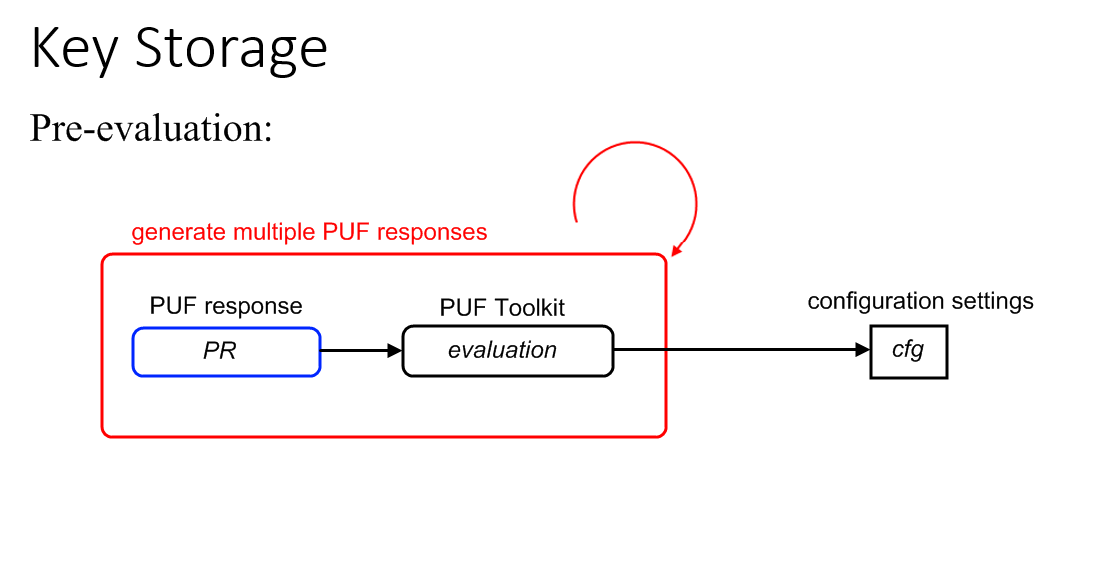
\includegraphics[width=0.8\textwidth]{images/BCH_pre-evaluation.png}}
\caption{Conceptual design of the pre-evaluation phase for a PUF-based secure key storage.}
\label{img:fz_1}
\end{figure}
The influence of noise and other environmental conditions can be pre-evaluated, so a selection of competent error correction algorithms can be optimized and an efficient implementation of a fuzzy extractor to regulate the variations can be established. Most implementations of fuzzy extractors utilize a static approach, which implies that the enlisted error correction code has a static maximum error
correction capability. The Golay (23, 12, 7) code can correct up to three errors but the environmental factors like aging effects render this code useless because they can introduce more errors than expected, so in the thesis, BCH code is also used as a building block in the fuzzy extractor. There are three major steps to implement a secure key recovery using a Fuzzy extractor. In the first phase we discard the unreliable PUF bits to reduce the burden on the error correction scheme that is called
Prevaluation. The second phase is called generation/enrollment followed by the reproduction phase.\\

\textbf{Pre-evaluation}: The PUF response properties are evaluated in this step. Some parameters that affect the PUF instance are static and remain constant with different PUF response generations, so measurements can be compensated for these parameters. Pre-evaluating the response also gives insight into the instensity of noise disturbance that can occur, consequently a BCH mode can be selected to adapt and correct errors instilled in the PUF-response by that noise. The conceptual
design for this phase is illustrated in Figure \ref{img:fz_1}.\\

\begin{figure}[htp]
\centering
\fbox{ 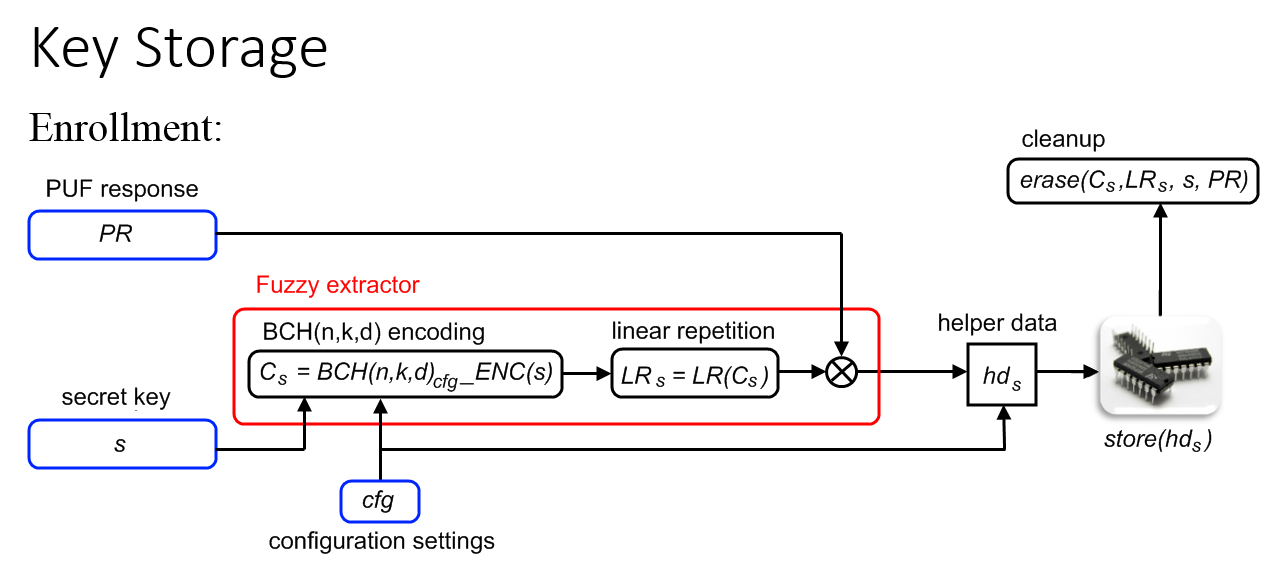
\includegraphics[width=0.97\textwidth]{images/BCH_KeyStorage_Enrollment.png}}
\caption{Conceptual design of the enrollment phase for a PUF-based secure key storage.}
\label{img:fz_2}
\end{figure}

\textbf{Generation}: The second phase also called the enrollment phase. It takes the secret key $s$, to be stored in the PUF-based secure key storage, and generates the matching helper data $hd_s$. The design for the generator is depicted in Figure \ref{img:fz_2}  The secret $s$ is provided as input to the BCH (n, k, d) encoder that is configurable via the input line \emph{cfg}, this results in the output of BCH encoded codewords $C_s$, since we are using systematic encoding BCH algorithm this means that
the encoded secret $s$ is contained in the codevectors. We denote this encoding for a certain configuration \emph{`cfg'} by $BCH(n,k,d)_{cfg}\_ENC(s) = C_s$. The configuration is decided in the \emph{pre-evaluation} phase, by setting the BCH code parameters $m, t$ and $n$.
Only the non-secret part (part of the output from BCH encoder that does not contains secret $s$) is taken from the codeword $C_s$ and a linear repetition code LR is applied to it to generate $LR_s$, denoted in the text as $LR_s = LR(C_s)$. In the end, helper data $hd_s$ for the secret key $s$ is derived by XORing the PUF response PR and $LR_s$ along with the configuration settings concatenated to the XORed result. This process is expressed in an equation as $hd_s = (PR \xor LR_s) \cup cfg$.
The helper data is stored in the non-volatile memory of the hardware device:$store(hd_s)$. The last step in this phase is cleanup where all the generated values $C_s, LR_s and PR$ are erased.\\

\begin{figure}[htp]
\centering
\fbox{ 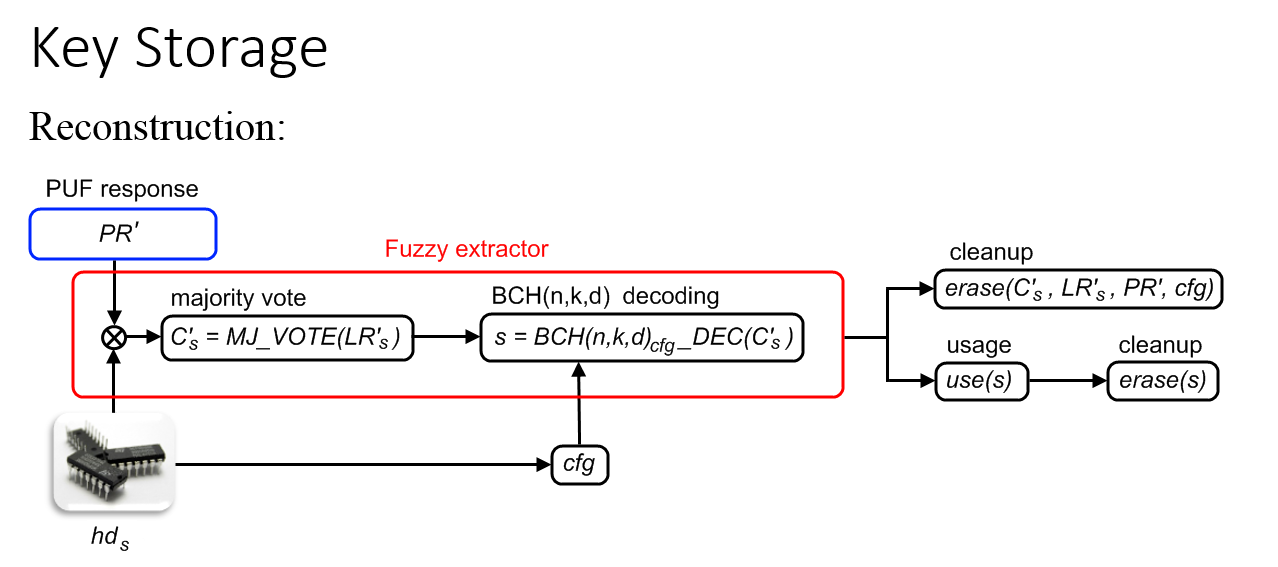
\includegraphics[width=0.97\textwidth]{images/BCH_KeyStorage_Reconstruction.png}}
\caption{Conceptual design of the reconstruction phase for a PUF-based secure key storage.}
\label{img:fz_3}
\end{figure}

\textbf{Reconstruction}: After storing the key as helper-data the same secret key $s$ must be restored. First, the `cfg' setting that was appended to the end of the helper-data is stripped. A new PUF response from the same device $PR'$ is XORed with stripped helper-data $hd_s$ to get $LR'_s$: $LR'_s = PR' \xor (hd_s\\cfg)$. Next, a Majority vote algorithm is applied to $LR'$ from which the encoded codeword $C'_s$ is recovered: $C'_s = MJ\_VOTE(LR'_s)$. After this the
reconstruction of the secret key $s$ is done by feeding the obtained $C'_s$ in the BCH (n,k,d) decoder: $C'_s = BCH(n,k,d)_{cfg}\_DEC(C'_s)$. The last step is similar to the generation phase i.e the cleanup of $PR', cfg and LR'_s$. The reproduced secret key $s$ is also erased after usage. An illustration for the reconstruction design is depicted in Figure \ref{img:fz_3}.

